% =============================================================================
% International Journal of Advanced Science and Engineering (IJASE)
% Mahendra Publications - Original Research Article
%
% Content: the Multiplicative Information Gating study previously prepared for
% TJEECS (see ../rejected-research-paper-8-tubitak). Every measured number,
% equation, proposition and proof is carried over unchanged. To meet the IJASE
% 15-page cap (which counts every table and figure as a full page) the prose is
% condensed, the conceptual pipeline schematic is dropped, and the illustrative
% headline decomposition is stated inline instead of as a separate table page.
%
% IJASE Guide for Authors compliance:
%   - A4, 12 pt standard font, double spacing, wide (3 cm) margins
%   - NO full justification (ragged right), every paragraph indented
%   - Numbered sections (1, 1.1, 1.1.1); Results and Discussion combined
%   - Abstract 100-150 words; max 5 keywords; Highlights as a SEPARATE file
%   - Conclusions <= 100 words; max 35 references for an original research paper
%   - References numbered in order of first appearance, [n] in text
%   - Figure captions listed separately; tables and figures each on their own
%     page at the END of the manuscript
%   - Maximum 15 pages in total, including text, references, tables and figures
% =============================================================================
\documentclass[12pt,a4paper]{article}

\usepackage[a4paper,margin=3cm]{geometry}      % IJASE: wide 3 cm margins
\usepackage{times}                              % standard serif font
\usepackage[T1]{fontenc}
\usepackage[utf8]{inputenc}
\usepackage{setspace}
\usepackage{indentfirst}                        % indent first paragraph of each section
\usepackage{amsmath,amssymb,amsthm}
\usepackage{booktabs}
\usepackage{array}
\usepackage{graphicx}
\usepackage{caption}
\usepackage{cite}                               % sort + compress [22-24] citation runs
\usepackage{ragged2e}                           % ragged right *with* hyphenation
\usepackage[hidelinks]{hyperref}
\usepackage{url}
\usepackage{tikz}
\usepackage{pgfplots}
\pgfplotsset{compat=1.17}

\captionsetup{font=small,labelfont=bf,labelsep=period}

% Body text stays double spaced (IJASE requirement). Only the *inter-block* glue
% around headings and displayed equations is tightened, which setspace otherwise
% inflates by the 1.667 stretch factor and which does not affect line spacing.
\usepackage{titlesec}
\titlespacing*{\section}{0pt}{0.55\baselineskip}{0.15\baselineskip}
\titlespacing*{\subsection}{0pt}{0.45\baselineskip}{0.05\baselineskip}
\setlength{\abovedisplayskip}{6pt}
\setlength{\belowdisplayskip}{6pt}
\setlength{\abovedisplayshortskip}{4pt}
\setlength{\belowdisplayshortskip}{4pt}

% Numbered headings: 1.  1.1  1.1.1
\renewcommand{\thesection}{\arabic{section}.}
\renewcommand{\thesubsection}{\arabic{section}.\arabic{subsection}}
\renewcommand{\thesubsubsection}{\arabic{section}.\arabic{subsection}.\arabic{subsubsection}}

% Propositions
\newtheorem{proposition}{Proposition}

\title{\textbf{Multiplicative Information Gating: Decomposing News into Novelty,
Materiality and Polarity for Calibrated Selective Forecasting}}

\author{
Anandkumar Pardeshi\,$^{a,*}$ \quad and \quad Sujata Deshmukh\,$^{b}$\\[0.5em]
\small $^{a}$Department of Computer Science and Engineering,
Fr.\ C.\ Rodrigues Institute of Technology,\\
\small Vashi, Navi Mumbai 400703, Maharashtra, India\\[0.2em]
\small $^{b}$Department of Computer Engineering,
Fr.\ C.\ Rodrigues Institute of Technology,\\
\small Vashi, Navi Mumbai 400703, Maharashtra, India\\[0.3em]
\small $^{*}$Corresponding author. E-mail: \texttt{anand.pardeshi@fcrit.ac.in}\\
\small Tel.: +91-22-2768-0000
}
\date{}

% =============================================================================
\begin{document}
\maketitle

% IJASE: ragged right (no constant right margin); keep paragraph indentation.
\RaggedRight
\setlength{\parindent}{1.27cm}
\setlength{\parskip}{0pt}
\doublespacing

% ---------- Abstract (100-150 words, no references) ----------
\begin{abstract}
\normalsize\noindent
Systems that turn text into decisions usually reduce each event to one sentiment
polarity and sum, conflating three properties that move prices through different
channels. We propose multiplicative information gating: an event is decomposed
into polarity, novelty and materiality and combined as their product, so any
near-zero factor vetoes the signal. We prove the product is the canonical combiner
under per-axis scaling and bound the signal by its weakest factor. A language model
supplies the three scores; the gated signal feeds a forecaster that is calibrated
and then permitted to abstain. On a live ledger of 621 resolved forecasts, nominal
90\% intervals covered 70.7\%. An offline three-stage recalibration cut expected
calibration error from 0.35 to 0.05. Single-name direction proved unpredictable
beyond drift at 50.1\%, so a conviction gate abstaining on 94\% of cases raised the
thirty-day hit rate to 60.6\% against a 58.0\% base.
\end{abstract}

\noindent\textbf{Keywords:} Calibration; Selective prediction; Sentiment
analysis;\\ Large language model; Financial forecasting

% ---------- Highlights ----------
% IJASE requires Highlights to be submitted as a SEPARATE file, not carried in the
% manuscript body. They live in Highlights.txt alongside this file.

% =============================================================================
\section{Introduction}
% =============================================================================

A growing class of decision systems reads text and acts on it. The dominant recipe
scores each item for sentiment polarity, averages the scores and feeds the average
to a predictor \cite{tetlock2007,loughran2011}, an approach that has shown media
tone to carry return-relevant information \cite{tetlock2007,antweiler2004}. Polarity
answers only one question, though: is this good or bad? It says nothing about
whether the news is new or a restatement of something priced weeks ago, nor whether
it bears on value or is merely cosmetic, so summed, loud and empty items drown out
the rare informative ones.

We therefore take a textual event to have three separable properties, each governing
price impact through a different channel: \emph{polarity}, the sign of the implied
value change; \emph{novelty}, how much genuinely new information it carries; and
\emph{materiality}, how sensitive fundamental value is to the event, independent of
sign or freshness. Multiplicative information gating combines them as a product,
which behaves like a soft logical AND: a stale or immaterial item yields a signal
near zero however strong its polarity, so one weak factor vetoes the event.

Who supplies the scores? Dictionaries capture polarity passably
\cite{loughran2011} but struggle with novelty and materiality, which require world
knowledge; we use an instruction-tuned large language model prompted with numerical
anchors \cite{brown2020,lopezlira2023}. And how do we keep the forecaster honest?
One near the efficient-market limit \cite{fama1970} is mostly wrong about direction,
so it owes the user a calibrated probability and the discipline to abstain when
conviction is low \cite{chow1970,geifman2017}. Our objectives are to formalise the
decomposition and its properties (Sections~2.1 and 3), to give a reproducible
scoring protocol (Section~2.2), and to couple the gated signal to a calibrated
selective forecaster, reporting measured results only (Section~4).

\subsection{Related work}

Tetlock \cite{tetlock2007} linked pessimistic media tone to downward pressure and
reversal, Antweiler and Frank \cite{antweiler2004} studied message boards, and
Loughran and McDonald \cite{loughran2011} showed finance-specific dictionaries
matter because general-purpose ones mislabel domain terms. Supervised text models
improve on dictionaries \cite{ke2019} and pre-trained language models now dominate
sentiment extraction \cite{huang2023}, but all treat the per-item output as a scalar
polarity, handling novelty and materiality by ad hoc filters if at all. Boudoukh et
al.\ \cite{boudoukh2019} is an exception in spirit: identifying which news is
relevant sharply changes the measured information content.

Instruction-tuned models emit structured numeric judgements from rubric-style
prompts \cite{brown2020} and finance has adopted them quickly \cite{lopezlira2023},
though their self-reported confidence is imperfectly calibrated
\cite{steyvers2025}. We do not ask the model to forecast but to \emph{decompose}, a
narrower and more checkable task; to our knowledge no prior work scores novelty and
materiality as separate, continuous per-item quantities and makes them
multiplicative preconditions for influence with a provable veto, existing pipelines
\cite{loughran2011,lopezlira2023,ke2019,huang2023} reducing the item to one polarity
first. Modern classifiers are often miscalibrated \cite{guo2017}; remedies include
Platt scaling \cite{platt1999} and isotonic regression \cite{zadrozny2002}, assessed
by expected calibration error and the Brier score \cite{brier1950}, while stacked
generalisation \cite{wolpert1992} complicates this, a failure we repair in
Section~2.3. Abstention is an old idea \cite{chow1970} with a modern theory
\cite{geifman2017} and a distribution-free cousin in conformal prediction
\cite{angelopoulos2021}. Financial machine learning is dominated by accuracy and
area-under-the-curve reporting, fragile under backtest overfitting
\cite{bailey2017}; deep and ensemble models are standard \cite{gu2020}, but few
report whether their probabilities are trustworthy.

% =============================================================================
\section{Materials and Methods}
% =============================================================================

\subsection{The multiplicative information model}

Let $e$ denote a textual event (a news headline) about an entity (a listed equity),
with scores $s(e)\in[-1,1]$ (polarity), $\nu(e)\in[0,1]$ (novelty, surprise relative
to the market's prior) and $\mu(e)\in[0,1]$ (materiality, the sensitivity of value
to the event regardless of sign). The \emph{event signal} is their product,
\begin{equation}
a(e) \;=\; s(e)\,\nu(e)\,\mu(e)\;\in[-1,1].
\end{equation}
Define \emph{relevance} $r(e)=\nu(e)\,\mu(e)$, so $a(e)=s(e)\,r(e)$. To aggregate
the events $\mathcal{E}$ touching one entity we use a relevance-weighted mean
restricted to events clearing a materiality floor $\mu_0$,
\begin{equation}
A \;=\; \frac{\sum_{e\in\mathcal{E}:\,\mu(e)\ge\mu_0} r(e)\,a(e)}
{\sum_{e\in\mathcal{E}:\,\mu(e)\ge\mu_0} r(e)}\;=\;\frac{\sum r(e)^2\,s(e)}{\sum r(e)}.
\end{equation}
Relevance enters twice, inside the event signal and again as the weight, so a novel
and material item dominates quadratically while cosmetic chatter is suppressed; we
use $\mu_0=0.15$. To first order the expected move is the product of a sign, a
sensitivity and a surprise magnitude; additive sentiment keeps only the sign, which
is why it over-reacts to loud, stale or immaterial items.

\subsection{Scoring the three axes with a language model}

The scores come from an instruction-tuned large language model (in our deployment,
Claude Haiku 4.5) prompted as a quantitative analyst and constrained to return a
JSON array of $\{\nu,\mu,s\}$ triples, one per headline, in input order. Two choices
make them reproducible. First, the prompt fixes \emph{numerical anchors} per axis:
for novelty, $0.0$ is an exact restatement of news priced weeks ago, $0.2$ an
in-line result, $0.6$ an unexpected but modest development and $1.0$ a sudden
regulatory ban; for materiality, $0.0$ is boilerplate, $0.4$ a contract worth a few
percent of revenue, $0.8$ a transformative deal and $1.0$ an existential event; for
polarity, anchors run from $-1.0$ (fraud allegation) through $0.0$ (a neutral
reshuffle) to $+1.0$ (a large earnings beat). Anchoring makes two runs on the same
item agree closely, which matters because the product in Eq.~(1) amplifies
disagreement on any one axis. Second, every scored item is memoised in a
content-addressed store keyed by a hash of the entity and normalised headline, so a
run is deterministic. When the model is unavailable, a lexicon fallback assigns
polarity from curated term lists with fixed conservative novelty and materiality,
flagged for downstream discounting.

\subsection{From gated signal to calibrated probability}

The aggregate $A$ of Eq.~(2) is one feature among several entering a hybrid
forecaster blending a gradient-boosted tree ensemble with a recurrent sequence model
over price, momentum, trend, reversal and volatility features, producing per name
and horizon a point forecast, a price interval and a directional probability
$\hat p$. We treat it as a black box and study its calibration, measured by the
expected calibration error over $B$ equal-width bins,
\begin{equation}
\mathrm{ECE}=\sum_{b=1}^{B}\frac{|G_b|}{N}\,\big|\,\overline{y}_b-\overline{p}_b\,\big|,
\end{equation}
with $\overline{p}_b$, $\overline{y}_b$ the mean predicted probability and mean
realised outcome in bin $b$, and by the Brier score
$\frac1N\sum_i(\hat p_i-y_i)^2$ \cite{brier1950}. Our first deployed model reported
a next-day up-probability near $0.80$ against a realised accuracy near $0.51$. The
cause was a stacking domain mismatch \cite{wolpert1992}: an isotonic calibrator
fitted on the out-of-fold \emph{average of the base learners} was applied to the
\emph{stacked} prediction, a different distribution, and the blend was never itself
calibrated. The repair is a three-stage calibration: refit the isotonic map on the
base-average it was meant to correct, form the blend, then fit a final Platt scaler
\cite{platt1999} on a held-out fold and apply it to the test and live rows.

\subsection{The conviction gate: abstention as decision-stage gating}

Calibration makes $\hat p$ honest, not skilful. If short-horizon direction is
near-random (Section~4.3), a calibrated probability sits near the base rate almost
everywhere and acting on every name is pointless. The remedy mirrors the text-stage
veto: act only when conviction clears a threshold. For a horizon of $H$ trading days
we emit an UP call when $\hat p\ge\tau^\star$ and NEUTRAL otherwise, choosing
$\tau^\star$ on training folds as the smallest $\tau$ whose fired bucket reaches a
target precision ($0.60$) while still firing at least a minimum fraction of the time
($5\%$):
\begin{equation}
\tau^\star=\min\Big\{\tau:\ \operatorname{prec}(\tau)\ge 0.60\ \text{and}\
\phi(\tau)\ge 0.05\Big\},
\end{equation}
where $\operatorname{prec}(\tau)=\Pr[y=1\mid \hat p\ge\tau]$ is the fired-bucket
precision and $\phi(\tau)=\Pr[\hat p\ge\tau]$ the firing rate. The gate is
intentionally one-sided: confident DOWN calls are destroyed by the upward drift of
equities (Section~4.4), so the system emits long-or-neutral signals only. Like the
event veto, it forgoes breadth for dependability, so the quantity worth reporting is
precision at a given firing rate, not accuracy or area under the curve.

\subsection{Data, deployment and evaluation protocol}

The system is deployed on liquid National Stock Exchange of India (NSE)
large-capitalisation equities, and two bodies of evidence are kept strictly
separate. The first is an \emph{offline walk-forward} study on daily data from 2018
to 2026 for a 54-name universe; all offline statistics are out-of-sample under an
expanding window, so no future information enters a fitted fold. The second is a
\emph{live append-only ledger}: since April 2026 the system has written every issued
forecast (entity, timestamp, target date, point forecast, interval, nominal
confidence, directional probability, horizon) to a row later stamped with the
realised price and outcome, scored first-look and never retro-edited.

% =============================================================================
\section{Theory}
% =============================================================================

The multiplicative form carries a guarantee no additive combiner offers.
\vspace{-0.3\baselineskip}

\begin{singlespace}
\begin{proposition}[Veto bound]
For every event $e$, $\;|a(e)| \le \min\{\,|s(e)|,\ \nu(e),\ \mu(e)\,\}$. In
particular $a(e)=0$ whenever any single factor is zero, and the aggregate satisfies
$|A|\le \max_{e}|s(e)|$.
\end{proposition}

\begin{proof}
Each factor lies in $[-1,1]$ with $\nu,\mu\ge 0$, so
$|a(e)|=|s(e)|\,\nu(e)\,\mu(e)$ is a product of three numbers of modulus at most
one; such a product cannot exceed the modulus of any one of them, which gives the
per-event bound and the zero case. For the aggregate, Eq.~(2) gives
$A=\big(\sum_e r(e)^2 s(e)\big)/\big(\sum_e r(e)\big)$, so
\[
|A|\;\le\;\frac{\sum_e r(e)^2\,|s(e)|}{\sum_e r(e)}\;\le\;\max_e|s(e)|\;\cdot\;
\frac{\sum_e r(e)^2}{\sum_e r(e)}\;\le\;\max_e|s(e)|,
\]
where the last step uses $\sum_e r(e)^2\le\big(\max_e r(e)\big)\sum_e r(e)\le\sum_e
r(e)$ because every $r(e)\in[0,1]$. The weights are non-negative but sub-stochastic,
so the aggregate contracts the polarities toward zero and never amplifies them.
\end{proof}
\end{singlespace}

Proposition~1 formalises ``a single weak factor vetoes the event'': a stale
($\nu\!\to\!0$) or immaterial ($\mu\!\to\!0$) item is capped near zero however
extreme its polarity. No additive combination does this, since a weighted sum
$\alpha s+\beta\nu+\gamma\mu$ is generally nonzero when one term vanishes.

\begin{singlespace}
\begin{proposition}[Characterisation]
Consider combiners $f(s,\nu,\mu)$ with $s\in[-1,1]$, $\nu,\mu\in[0,1]$ satisfying:
(A0) \emph{normalisation}, $f(1,1,1)=1$; (A1) \emph{sign fidelity},
$\operatorname{sign} f=\operatorname{sign} s$; (A2) \emph{veto}, $f=0$ if any of
$|s|,\nu,\mu$ is $0$; (A3) \emph{separable monotonicity}, $|f|$ is non-decreasing in
each of $\nu$ and $\mu$ for fixed others, and $f$ is non-decreasing in $s$ for fixed
$\nu,\mu\ge0$; and (A4) \emph{factor homogeneity}, scaling any single argument by
$\lambda\in[0,1]$ scales $f$ by $\lambda$. Then $f(s,\nu,\mu)=s\,\nu\,\mu$.
\end{proposition}

\begin{proof}[Proof sketch]
By (A4) applied to each argument in turn, scaling the arguments by $\lambda_1$,
$\lambda_2$, $\lambda_3$ in $[0,1]$ scales $f$ by $\lambda_1\lambda_2\lambda_3$.
Writing
$s=\operatorname{sign}(s)\,|s|$ and taking $\lambda_1=|s|$, $\lambda_2=\nu$,
$\lambda_3=\mu$ relative to the unit corner gives
$f(s,\nu,\mu)=|s|\,\nu\,\mu\,f(\operatorname{sign}(s),1,1)$. Sign fidelity (A1)
forces $f(\pm1,1,1)=\pm c$ with $c=f(1,1,1)$, and normalisation (A0) fixes $c=1$.
Hence $f=s\,\nu\,\mu$; (A2) and (A3) are then automatically satisfied, so they are
consistency requirements rather than the active constraints.
\end{proof}
\end{singlespace}

The force of the result lies in homogeneity (A4): it requires each axis to act on
its own multiplicative scale, and once that and (A0) are granted the product
follows. Since (A2) and (A3) do not by themselves single out the product, we claim
only that it is the canonical combiner once per-axis scaling is imposed --- exactly
what a position-taking system needs to treat freshness and relevance as
preconditions for influence.

% =============================================================================
\section{Results and Discussion}
% =============================================================================

\subsection{Deployed uncertainty does not self-correct}

Between 19 April and 12 June 2026 the system issued and later resolved 621
price-interval forecasts on seven NSE large caps (ABB, HDFCBANK, ICICIBANK, INFY,
RELIANCE, SBIN, TCS), each carrying a nominal $90\%$ interval with a median
half-width of $5.6\%$ of price. Had the intervals been well calibrated, about $90\%$
would contain the realised price; empirical coverage was $70.7\%$ overall, a $19.3$
percentage-point shortfall. Most forecasts were at the ten-day horizon, where
coverage was $69.2\%$ over 575 resolved forecasts; the smaller twenty-day and
five-day buckets covered $86.8\%$ and $100\%$ (Table~1a, Figure~1a). Stated confidence
was systematically overstated and nothing in the pipeline noticed: the empirical
reason calibration and abstention cannot be afterthoughts.

\subsection{A stacking domain mismatch, and a three-stage repair}

This and the two results that follow are walk-forward measurements, not live-ledger
figures. The original next-day directional head reported probabilities clustered
near $0.80$ against a realised accuracy of about $0.51$, giving
$\mathrm{ECE}=0.345$ and a Brier score above $0.366$, worse than always predicting
$0.5$. The three-stage repair of Section~2.3 cut ECE from $0.345$ to $0.049$ and
pulled the reported up-probability back to a realistic neighbourhood of $0.50$.
Accuracy did not move: calibration changed what the model \emph{said about its
confidence}, not what it predicted. A calibrator is bound to the distribution it was
fitted on, and stacking creates more than one.

\subsection{Single-name direction is unpredictable beyond drift}

With probabilities pulled back to the base rate, we asked whether any single-name
directional edge survives at short horizons. A cross-sectional model predicting
five-day direction reached $50.09\%$ out-of-fold accuracy, with a ranking area under
the curve near $0.49$; that is chance. We confirmed this five ways, varying the
learner and feature set and gating by trend and market regime; none produced a
stable edge over the always-up base rate. This matches the efficient-market
prediction for liquid names \cite{fama1970} and reframes the problem: if ordering
names by predicted return is near-random, the only lever left is \emph{selection}.

\subsection{Selection recovers a small, stable edge}

Lengthening the horizon to thirty trading days opens two modest edges: the upward
drift of equities (about $58\%$ of thirty-day windows are up) and a small
idiosyncratic component captured by a calibrated cross-sectional model on momentum,
trend, reversal and volatility features. Walk-forward from 2018 to 2026 over the
54-name universe (91{,}471 training rows, 50{,}272 out-of-sample rows), the gate of
Eq.~(4) settles at $\tau^\star=0.63$. The fired UP bucket achieves $60.6\%$
directional precision against a $58.0\%$ always-up base rate, a net edge of $2.6$
percentage points, while firing on only $5.6\%$ of observations; the model abstains
on the remaining $94\%$. The bucket pools to $2{,}840$ calls, so the $60.6\%$
precision carries a $95\%$ binomial interval of $58.8$ to $62.4\%$, and a one-sided
test against the base gives $z\approx2.9$ ($p\approx0.002$). We do not over-read it:
per-year fired counts are small (Table~1b), so the swings from $+10.8$ points in 2025
to $-2.4$ in 2024 are within sampling noise, and the honest summary is a small but
repeatable tail edge. The ranking area under the curve is about $0.47$: the edge
lives in the high-conviction tail, not the ordering, which is what precision at a
fixed firing rate registers and area under the curve overlooks. The gate beats its
base rate in four of five test years (Table~1b, Figure~1b). Confident DOWN calls
reach only about $10\%$ precision out-of-sample, destroyed by drift, which is why
the gate never emits them.

\subsection{The veto in action}

The text stage cannot be evaluated as an isolated alpha, because the deployed ledger
stores no per-event return labels; what we can show is that the decomposition
behaves as designed. Scoring four headlines for one entity under the anchors of
Section~2.2 gives $a=+0.018$ for a consensus-meeting profit in an upbeat tone
($s=+0.30$, $\nu=0.20$, $\mu=0.30$), $+0.022$ for a reiterated buyback ($+0.55$,
$0.10$, $0.40$) and $+0.003$ for a routine reshuffle ($+0.05$, $0.40$, $0.15$), but
$-0.330$ for an unexpected regulator notice on a core product line ($-0.55$, $0.75$,
$0.80$). The glowing but routine item and the emphatic but cosmetic one are gated
down an order of magnitude, while the quieter disclosure that is new and material
dominates despite its moderate polarity --- the protection Proposition~1 guarantees
and additive sentiment cannot. These values illustrate scoring behaviour and carry
no performance claim.

\subsection{Discussion, threats to validity and honest limits}

Every result turns on one trade-off: the text-stage veto refuses stale or immaterial
items and the decision-stage gate stays out on most names, so the system gives up
commenting on everything and earns the right to be believed on the little it flags.
Nothing in Section~2 is specific to equities: any stream of timestamped textual
events driving a decision has the same three axes, and triage of clinical alerts,
operations tickets and moderation queues fail the same way when collapsed to one
urgency score. The gate is an instance of selective classification
\cite{chow1970,geifman2017}, paired here with a probability whose calibration was
repaired; distribution-free interval methods \cite{angelopoulos2021} address the
coverage failure of Section~4.1.

Four limits deserve emphasis. The language-model scores are judgements, not
measurements: anchoring tightens them but a different model or prompt could shift
the scale. The live ledger is young --- two months and seven names --- so its
coverage shortfall is a snapshot, not a stationary law. Weightiest, we have no
per-event return labels in deployment, so the marginal value of the decomposition
over plain polarity is argued from its formal properties and its place in the
measured pipeline rather than an isolated backtest, which would invite the
backtest-overfitting critique \cite{bailey2017}. Finally, the live
directional-probability sample is small, 28 resolved next-period calls, so our live
claim rests on the 621-forecast interval-coverage evidence.

% =============================================================================
\section{Conclusions}
% =============================================================================

A textual event carries direction, surprise and consequence, and these need not move
together; their product builds a signal whose weakest axis caps the rest, keeping a
live decision from chasing loud noise, and it is the canonical combiner once
per-axis scaling is imposed. The same logic belongs at the decision stage: nominal
$90\%$ intervals covered only $70.7\%$ of live outcomes, a three-stage recalibration
cut expected calibration error from $0.35$ to $0.05$, and a conviction gate
abstaining on $94\%$ of names raised the thirty-day hit rate to $60.6\%$ against a
$58.0\%$ base.

% =============================================================================
\section{Acknowledgements}
% =============================================================================

The authors thank the Department of Computer Engineering, Fr.\ C.\ Rodrigues
Institute of Technology, for computing support. No external funding was received and
the authors declare no conflict of interest.

\noindent\textbf{Declaration of generative AI.} An instruction-tuned model (Claude
Haiku 4.5, Anthropic) is used as a measurement instrument within the system under
study, scoring headlines from the anchored prompt of Section~2.2; those outputs were
validated against the deterministic fallback and persisted for audit. During
manuscript preparation a large language model was used solely to improve language
and readability; no generative tool produced data, results, figures or
interpretations, and the authors take full responsibility.

\noindent\textbf{Data availability.} The live forecast ledger and the offline
walk-forward statistics underlying Table~1 and Figure~1 are available from the
corresponding author on reasonable request. Price data are public NSE end-of-day
records.

% =============================================================================
\section{References}
% =============================================================================
\renewcommand{\refname}{}
\vspace{-2\baselineskip}
\begin{singlespace}
\begin{thebibliography}{99}
\setlength{\itemsep}{0pt}
\setlength{\parskip}{0pt}

\bibitem{tetlock2007}
Tetlock, P.C., 2007. Giving content to investor sentiment: the role of media in the
stock market. Journal of Finance, 62, 1139--1168.

\bibitem{loughran2011}
Loughran, T., McDonald, B., 2011. When is a liability not a liability? Textual
analysis, dictionaries, and 10-Ks. Journal of Finance, 66, 35--65.

\bibitem{antweiler2004}
Antweiler, W., Frank, M.Z., 2004. Is all that talk just noise? The information
content of internet stock message boards. Journal of Finance, 59, 1259--1294.

\bibitem{brown2020}
Brown, T.B., Mann, B., Ryder, N., et al., 2020. Language models are few-shot
learners. In: Adv. Neural Inf. Process. Syst. 33, pp. 1877--1901.

\bibitem{lopezlira2023}
Lopez-Lira, A., Tang, Y., 2023. Can ChatGPT forecast stock price movements? Return
predictability and large language models. arXiv:2304.07619. [cited 2026 Aug 5].
Available from: \url{https://arxiv.org/abs/2304.07619}.

\bibitem{fama1970}
Fama, E.F., 1970. Efficient capital markets: a review of theory and empirical work.
Journal of Finance, 25, 383--417.

\bibitem{chow1970}
Chow, C.K., 1970. On optimum recognition error and reject tradeoff. IEEE
Transactions on Information Theory, 16, 41--46.

\bibitem{geifman2017}
Geifman, Y., El-Yaniv, R., 2017. Selective classification for deep neural networks.
In: Adv. Neural Inf. Process. Syst. 30, pp. 4878--4887.

\bibitem{ke2019}
Ke, Z.T., Kelly, B.T., Xiu, D., 2019. Predicting returns with text data. National
Bureau of Economic Research Working Paper 26186, Cambridge.

\bibitem{huang2023}
Huang, A.H., Wang, H., Yang, Y., 2023. FinBERT: a large language model for
extracting information from financial text. Contemporary Accounting Research, 40,
806--841.

\bibitem{boudoukh2019}
Boudoukh, J., Feldman, R., Kogan, S., Richardson, M., 2019. Information, trading,
and volatility: evidence from firm-specific news. Review of Financial Studies, 32,
992--1033.

\bibitem{steyvers2025}
Steyvers, M., Tejeda, H., Kumar, A., et al., 2025. What large language models know
and what people think they know. Nature Machine Intelligence, 7, 221--231.

\bibitem{guo2017}
Guo, C., Pleiss, G., Sun, Y., Weinberger, K.Q., 2017. On calibration of modern
neural networks. In: Proc. 34th Int. Conf. Mach. Learn., pp. 1321--1330.

\bibitem{platt1999}
Platt, J.C., 1999. Probabilistic outputs for support vector machines and comparisons
to regularized likelihood methods. In: Adv. Large Margin Classifiers. MIT Press, pp. 61--74.

\bibitem{zadrozny2002}
Zadrozny, B., Elkan, C., 2002. Transforming classifier scores into accurate
multiclass probability estimates. In: Proc. 8th ACM SIGKDD Int. Conf., pp. 694--699.

\bibitem{brier1950}
Brier, G.W., 1950. Verification of forecasts expressed in terms of probability.
Monthly Weather Review, 78, 1--3.

\bibitem{wolpert1992}
Wolpert, D.H., 1992. Stacked generalization. Neural Networks, 5, 241--259.

\bibitem{angelopoulos2021}
Angelopoulos, A.N., Bates, S., 2023. A gentle introduction to conformal prediction
and distribution-free uncertainty quantification. Foundations and Trends in Machine
Learning, 16, 494--591.

\bibitem{bailey2017}
Bailey, D.H., Borwein, J., Lopez de Prado, M., Zhu, Q.J., 2017. The probability of
backtest overfitting. Journal of Computational Finance, 20, 39--69.

\bibitem{gu2020}
Gu, S., Kelly, B., Xiu, D., 2020. Empirical asset pricing via machine learning.
Review of Financial Studies, 33, 2223--2273.

\end{thebibliography}
\end{singlespace}

% =============================================================================
% IJASE: figure captions listed separately, then each table/figure on its own page
% =============================================================================
\clearpage
\section*{Figure Captions}
\begin{singlespace}
\noindent\textbf{Figure 1.} Measured behaviour of the two dependability mechanisms.
(a) Empirical coverage of nominal $90\%$ intervals on the live ledger by horizon
(resolved forecasts: 8, 575, 38, 621 in total). (b) Fired-bucket precision of the
conviction gate against the always-up base rate by test year, at about a $5.6\%$
firing rate.
\end{singlespace}

% ---------- Tables and figures, each on its own page ----------

\clearpage
\begin{table}[p]
\centering
\caption{Measured results. Panel (a): live-ledger interval coverage by horizon (NSE
large caps, 19 April--12 June 2026; every interval carries a nominal $90\%$ level).
Panel (b): walk-forward selective signal by test year, where precision is the
realised up-rate of the fired high-conviction bucket, base is the always-up rate and
fires is the number of high-conviction calls.}
\label{tab:results}
\begin{singlespace}
\small
\noindent\textbf{(a) Live-ledger interval coverage by horizon}\\[2pt]
\begin{tabular}{lccc}
\toprule
\textbf{Horizon} & \textbf{Resolved forecasts} & \textbf{Nominal} &
\textbf{Empirical} \\
\midrule
5 trading days  & 8   & 90.0\% & 100.0\% \\
10 trading days & 575 & 90.0\% & 69.2\%  \\
20 trading days & 38  & 90.0\% & 86.8\%  \\
\midrule
\textbf{All}    & \textbf{621} & \textbf{90.0\%} & \textbf{70.7\%} \\
\bottomrule
\end{tabular}

\vspace{1.4em}
\noindent\textbf{(b) Walk-forward selective signal by test year}\\[2pt]
\begin{tabular}{lcccc}
\toprule
\textbf{Test year} & \textbf{Fires} & \textbf{Fired precision} &
\textbf{Always-up base} & \textbf{Edge (pp)} \\
\midrule
2022 & 365 & 61.6\% & 54.0\% & $+7.6$ \\
2023 & 290 & 68.3\% & 65.3\% & $+3.0$ \\
2024 & 932 & 53.3\% & 55.7\% & $-2.4$ \\
2025 & 822 & 69.0\% & 58.2\% & $+10.8$ \\
2026 & 431 & 54.5\% & 47.1\% & $+7.4$ \\
\midrule
\textbf{Pooled} & \textbf{2{,}840} & \textbf{60.6\%} & \textbf{58.0\%$^{\dagger}$} &
\textbf{$+2.6$} \\
\bottomrule
\end{tabular}

\vspace{4pt}
{\footnotesize $^{\dagger}$The pooled base is the unconditional always-up rate over
all out-of-sample rows, not the fires-weighted mean of the yearly bases ($55.9\%$);
the pooled edge is therefore the conservative of the two comparisons.}
\end{singlespace}
\end{table}

\clearpage
\begin{figure}[p]
\centering
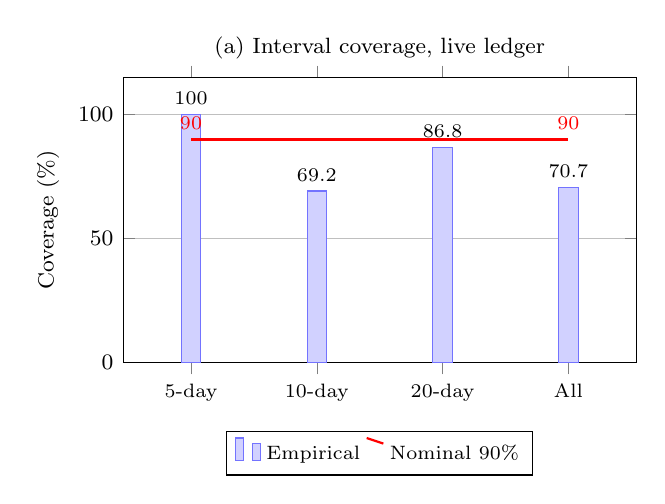
\begin{tikzpicture}
\begin{axis}[
  width=8.1cm, height=5.2cm, font=\footnotesize,
  ybar, bar width=7pt,
  symbolic x coords={5-day,10-day,20-day,All},
  xtick=data, x tick label style={font=\scriptsize},
  ymin=0, ymax=115, ylabel={Coverage (\%)},
  enlarge x limits=0.18, ymajorgrids,
  legend style={at={(0.5,-0.24)},anchor=north,legend columns=2,font=\scriptsize},
  nodes near coords, every node near coord/.append style={font=\scriptsize},
  title={(a) Interval coverage, live ledger}, title style={font=\footnotesize,yshift=-1mm}
]
\addplot[fill=blue!18,draw=blue!55] coordinates {(5-day,100.0)(10-day,69.2)(20-day,86.8)(All,70.7)};
\addplot[sharp plot,thick,red,mark=none,update limits=false] coordinates {(5-day,90)(All,90)};
\legend{Empirical, Nominal 90\%}
\end{axis}
\end{tikzpicture}

\vspace{10mm}

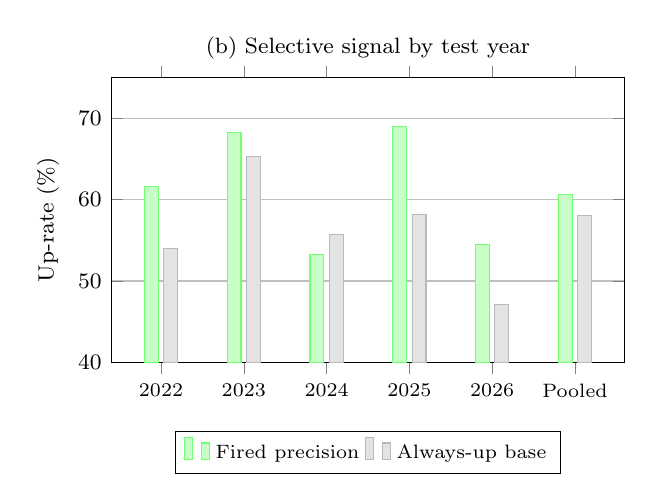
\begin{tikzpicture}
\begin{axis}[
  width=8.1cm, height=5.2cm, font=\footnotesize,
  ybar, bar width=5pt,
  symbolic x coords={2022,2023,2024,2025,2026,Pooled},
  xtick=data, x tick label style={font=\scriptsize},
  ymin=40, ymax=75, ylabel={Up-rate (\%)},
  enlarge x limits=0.12, ymajorgrids,
  legend style={at={(0.5,-0.24)},anchor=north,legend columns=2,font=\scriptsize},
  title={(b) Selective signal by test year}, title style={font=\footnotesize,yshift=-1mm}
]
\addplot[fill=green!22,draw=green!55] coordinates {(2022,61.6)(2023,68.3)(2024,53.3)(2025,69.0)(2026,54.5)(Pooled,60.6)};
\addplot[fill=gray!22,draw=gray!55] coordinates {(2022,54.0)(2023,65.3)(2024,55.7)(2025,58.2)(2026,47.1)(Pooled,58.0)};
\legend{Fired precision, Always-up base}
\end{axis}
\end{tikzpicture}
\caption{Measured behaviour of the two dependability mechanisms (see Figure
Captions).}
\label{fig:results}
\end{figure}

\end{document}
